\documentclass[10pt,a4paper]{amsart}
\usepackage[margin=19mm]{geometry}
\usepackage{amsmath,amssymb,mathtools}
\usepackage[scr=rsfs,cal=euler]{mathalfa}
\usepackage{xfrac}
\usepackage[unicode,hidelinks,bookmarks=false]{hyperref}
\newcommand{\ie}{i.e.\ }
\newcommand{\cf}{cf.\ }
\newcommand{\resp}{respectively\ }
\newcommand{\Subsection}{\subsection}
\providecommand{\nobreakdash}{\nobreak\hbox{-}}
\setlength{\emergencystretch}{2em}
\multlinegap0pt
\usepackage{tikz}
\usepackage{mathtools}
\usepackage{amssymb}
\usepackage[shortlabels]{enumitem}
\usepackage{dsfont}
\newtheorem{proposition}{Proposition}
\title{Cohomology rings and $p$-local behavior of even Artin groups.}
\author{Marcos Escart\'in Ferrer, Giorgio Leoni, Conchita Mart\'inez P\'erez}
\date{Source: arXiv:2606.30558v1 (CC BY 4.0)}
\begin{document}
\maketitle

\noindent\emph{Source and licence.} Cohomology rings and $p$-local behavior of even Artin groups.. Version arXiv:2606.30558v1 (CC BY 4.0), distributed by arXiv under the Creative Commons Attribution 4.0 International licence, http://creativecommons.org/licenses/by/4.0/, as recorded in the arXiv licence metadata for this exact version and shown on the abstract page https://arxiv.org/abs/2606.30558v1. Full licence notice: \texttt{licenses/arxiv-2606.30558-CC-BY-4.0.txt}.\par\smallskip

\noindent\textit{Editorial scope.} Counted unit: the article's proposition TriangleArtin (source0.tex lines 488--490). The article's complete original proof of it is delivered with it (source0.tex lines 492--518, one \texttt{proof} environment of 27 lines). No mathematics is written, repaired or re-derived: the statement and the proof are the article's own lines, in the article's own notation, and no retained line is substituted or re-flowed.  No further source-local context is needed: every cross-reference of every retained line resolves inside the two delivered spans.  Nothing was omitted from any retained span, so the package carries no omission record.  No retained line contains a citation, so the wrapper carries no bibliography and no bibliography entry.  The retained lines contain the article's own diagram code, which the wrapper typesets with the standard tikz packages; no image file is delivered and the package declares no asset dependency.  Editorial formatting only, in addition: an AMS \texttt{amsart} preamble that restates the article's own declarations and macros used by the retained lines, namely the environments \texttt{proposition} on separate counters, together with the standard packages those lines need.  The retained environments print in this document as Proposition 1 in order of appearance, whereas the article prints the same items with the numbering of its own full document.  The complete native source of the article as distributed in the arXiv e-print for this exact version is bundled unchanged as \texttt{sources/204033/source0.tex}.
\begin{proposition}\label{TriangleArtin}
If two triangular even Artin groups are isomorphic, then their defining graphs have the same number of edges labeled $2$.
\end{proposition}

\begin{proof}
Consider the group $A_\Omega$, where $\Omega$ is the following graph:
$$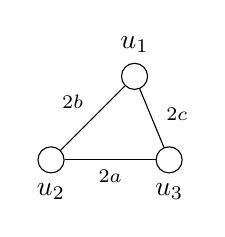
\begin{tikzpicture}[main/.style = {draw, circle},node distance={15mm}] 
    \node[label=below:{$u_2$}][main] (1)  {}; 
    \node[label={$u_1$}][main] (6) [above right of=1] {};
    \node[label=below:{$u_3$}][main] (2) [right of=1] {}; 
    
    \draw[-] (1) -- node[below] {$\scriptstyle{2a}$}  (2);
    \draw[-] (1) -- node[above left]{$\scriptstyle{2b}$}  (6);
    \draw[-] (6) -- node[pos=0.7,above right] {$\scriptstyle{2c}$}   (2);
\end{tikzpicture}$$
with $a,b,c\geq 2$. Then $S(A_\Omega)$ is the 2-sphere $\mathbb{S}^2$ and
$\mathrm{Liv}^\chi$ is disconnected if and only if one of the following holds:
\begin{itemize}
    \item $\chi(u_i)=0$ and $\chi(u_{i+1})+\chi(u_{i+2})=0$ for $i\in\{1,2,3\}$;
    \item $\chi(u_i)+\chi(u_{i+1})=0$ and $\chi(u_i)+\chi(u_{i+2})=0$ for $i\in\{1,2,3\}$,
\end{itemize}
where the indices are taken modulo $3$. In particular, $\Sigma^1(A_\Omega)$ is homotopy equivalent to $\mathbb{S}^2$ with $12$ points removed, so $\pi_1(\Sigma^1(A_\Omega))\cong F_{11}$. Similarly,  
\begin{enumerate}
    \item if $\Omega$ has precisely one edge labeled $2$, $\Sigma^1(A_\Omega)$ is $\mathbb{S}^2$ with $6$ points removed so $\pi_1(\Sigma^1(A_\Omega))\cong F_5$;

    \item  if $\Omega$ has precisely two edges labeled $2$, then $\Sigma^1(A_\Omega)$ is $\mathbb{S}^2$ with $2$ points removed so $\pi_1(\Sigma^1(A_\Omega))$ is cyclic and
    
   \item if all three edges of $\Omega$ are labeled $2$, then the group $A_\Omega$ is free abelian and  $\Sigma^1(A_\Omega)=S(A_\Omega)$.
\end{enumerate}
Therefore, the claim follows.
\end{proof}

\end{document}
